\documentclass[10pt,journal]{IEEEtran}
\usepackage[letterpaper, margin=0.8in]{geometry}
\usepackage{framed, listings, graphicx, float, amsmath,url}

\begin{document}

\title{
\includegraphics[width=0.4\linewidth]{figures/rewrite}}

\author{EE149/249A Project Report, Fall 2015

Reia Cho, CJ Geering, Nathaniel Mailoa, Rachel Zhang

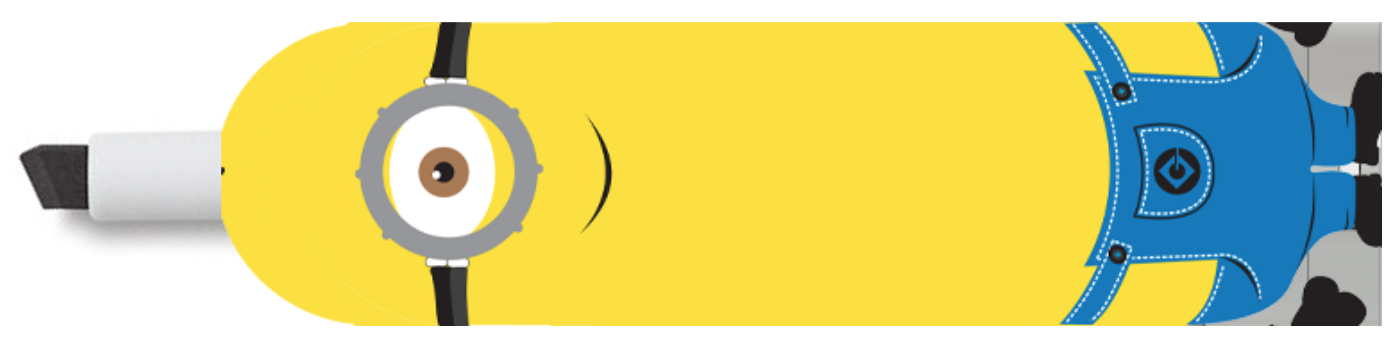
\includegraphics[width=0.45\linewidth]{figures/minion}}


% make the title area
\maketitle


\section{Introduction}
\par Slept through lecture again? Studying for an exam, but can't remember what the professor wrote during class? Can't make out what the professor is writing from the back of the classroom? Need to work out a problem on pen and paper over a Skype call? Have no fear, reWRITE is here!
\par reWRITE is a writing utensil attachment that aims to digitize handwriting in a self-contained, easy-to-implement, and cost effective manner. Digitizing handwriting is  a callenging open-problem with no single solution. Currently, there exist only a few solutions, each with their own benefits and tradeoffs. The most common solution currently uses an infrared tracking system. The writing utensil is equipped an IR transmitter whose signal is received by a distant IR camera elsewhere in the room. The main drawback with this type of system is that it lacks self-containment.
\par reWRITE is designed specifically for a classroom or presentation environment, both of which demand mobility and easy setup. Thus, we decided to use a single Inertial Measurement Unit (IMU) instead of the IR implementation. By having all sensors onboard, reWRITE is one single unit with no need for reciever or projector setup. Additionally, reWRITE is completely wireless in terms of power and communication.
\par reWRITE interprets IMU data and provides both real-time and historical handwriting data. Real-time data can be livestreamed using free streaming services such as YouTube and Twitch.tv. For those who are visually impaired or have trouble reading the board, opening up the stream to see the handwriting at any size is extremely convenient and sometimes necessary. reWRITE can also be used during a conference call to provide a common medium to exchange handwritten notes or drawings. In addition to live streaming, all of the data can be stored and revisited at any time.

\par A demo of the reWRITE can be found in \textit{\url{https://youtu.be/FYBg0k001e8}}.

\section{System}

\begin{figure}[H]
  \centering
    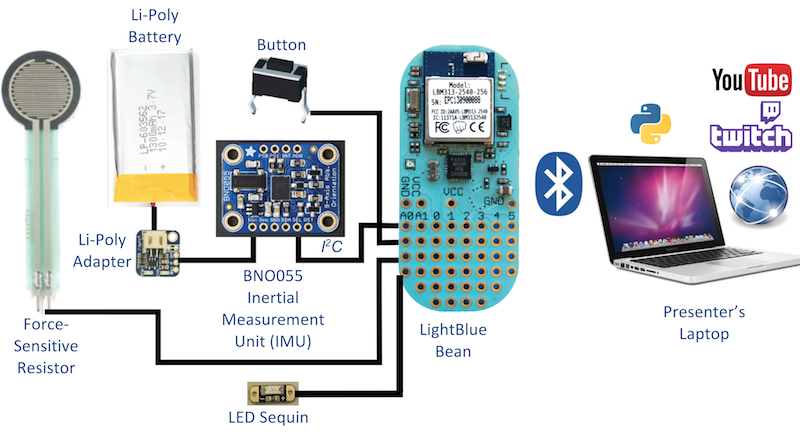
\includegraphics[width=\linewidth]{figures/system}
  \caption{reWRITE system}
  \label{fig:system}
\end{figure}

\subsection{LightBlue Bean}

\begin{figure}[H]
  \centering
    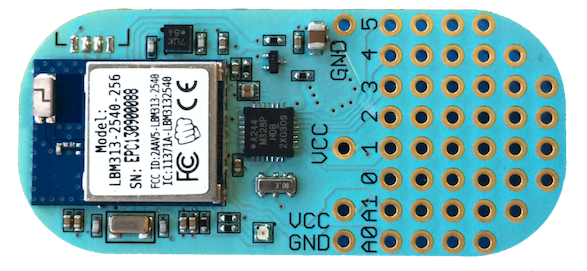
\includegraphics[width=0.8\linewidth]{figures/bean}
  \caption{LightBlue Bean}
  \label{fig:bean}
\end{figure}

For the main controller, we initially chose to use the RedBearLab BLE Nano, but ran into issues with the low level BLE protocol. Because the BLE Nano is typically used to communicate with a smartphone or other BLE modules, we had to develop an XCode project on OSX to use it with a PC.
The LightBlue Bean is a more reasonable platform. The Bean has an 8MHz ATMega328p microcontroller, a LightBlue LBM313 Bluetooth Low Energy (BLE) module, an RGB LED, a temperature sensor, and a 3-axis accelerometer. Unfortunately, it does not have a gyroscope, so we still need a separate IMU module. 
\par The Bean runs on a 3V CR2032 coin cell and also has a pin that can be used to provide power. The BLE connects to PCs wirelessly and is easy to program because LightBlue provides libraries for a virtual serial port. Because the Bean and Arduino Nano have similar functionalities and microcontrollers, we were able to port the Arduino code to the Bean without any compatibility issues.

\subsection{BNO055 Absolute Orientation Sensor Breakout Board}

\begin{figure}[H]
  \centering
    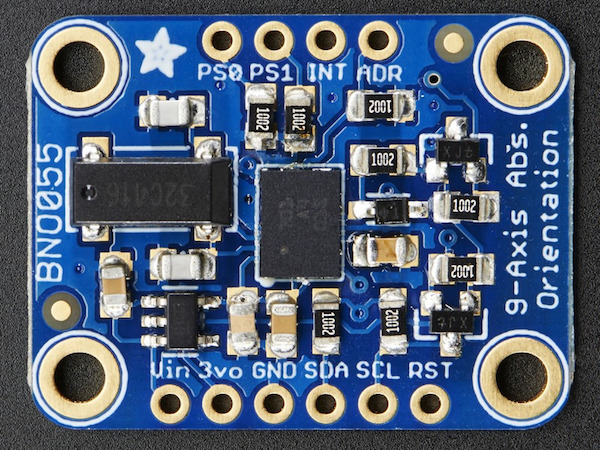
\includegraphics[width=0.6\linewidth]{figures/imu}
  \caption{BNO055 IMU breakout board}
  \label{fig:imu}
\end{figure}
  The BNO055 is a 9-Degree of Freedom Inertial Measurement Unit (IMU) that provides accelerometer, gyroscope, and magnetometer data. Running onboard the 32-bit M0+ microcontroller is the Bosch Sensortec sensor fusion algorithm that combines sensor data for calibration and filtering. We also used this device to send linear acceleration and Euler angles. The processed data is available at a datarate of 100Hz. The IMU communicates to the Bean through I2C in the Bean's analog pins.
\par When the device is initially powered, it must be calibrated. Each sensor is calibrated separately by the onboard microcontroller and a register in the device stores the calibration status for each sensor out of 3. The gyroscope is calibrated by keeping the IMU stationary. The magnetometer is calibrated by drawing a figure eight. To calibrate the accelerometer, the IMU must be stationary for a few seconds in various orientations. Overall, the three sensors take about 30 to 60 seconds to calibrate. To help with calibration, we use the Bean's RGB LED to signify the calibration status. Even after the IMU is fully calibrated, it is still not perfect, which we will discuss in the position reconstruction section.
\subsection{Li-Ion Battery}

\begin{figure}[h]
  \centering
    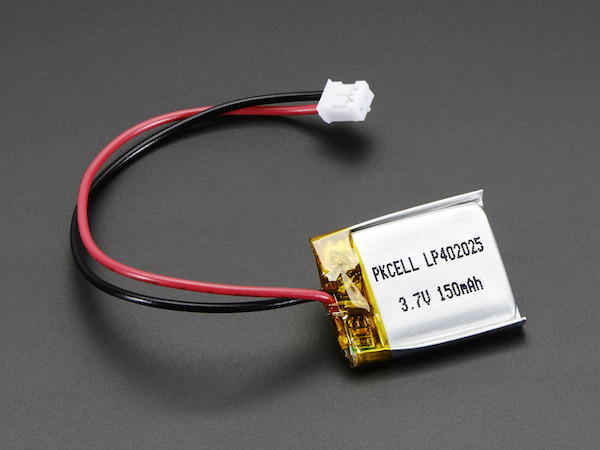
\includegraphics[width=0.6\linewidth]{figures/battery}
  \caption{3.7V 150mAh Li-Ion battery}
  \label{fig:battery}
\end{figure}
  To power our devices, we use a 3.7V 150 mAh Li-Ion battery with a breakout board because the small size fits the form factor of the reWRITE. The LightBlue Bean is hooked up to the battery through the IMU board because it needs a source between 3.0 to 3.6V and does not have an on-board regulator.

\subsection{Force Sensor}

\begin{figure}[H]
  \centering
    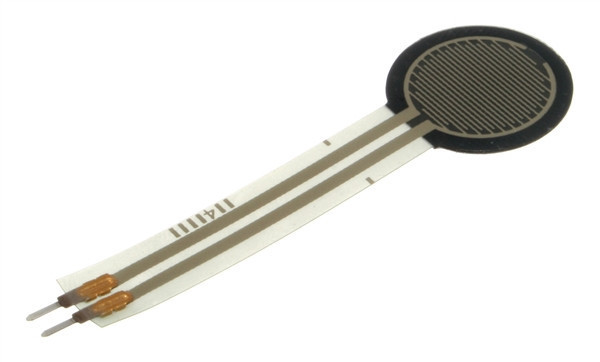
\includegraphics[width=0.6\linewidth]{figures/force-sensor}
  \caption{Force sensor}
  \label{fig:system}
\end{figure}
  To detect when someone is writing with the marker, we attached a force sensor to the back of the marker casing such that the marker pushes against it when writing. The force sensor is, effectively, a variable resistor -- about 8 K$\Omega$ when not pushed and about 2 K$\Omega$ when pushed. We used a resistive divider circuit and the digitalRead() function on the LightBlue Bean to determine when the marker was writing. A spring between the force sensor and the marker prevents the marker from constantly pushing against the force sensor.

\subsection{Button and LED Sequin}
  Our last two peripherals were a button and an LED Sequin. The LED Sequin, a tiny module containing a surface-mount LED and resistor, shows whether or not the force sensor is being pushed. The reWRITE also has a small tactile button hooked up to a resistive divider circuit. This lets the user signify that the marker was ready for position calibration (to establish a point of origin). It is also used to clear the plotting canvas in the reconstruction.

\section{Casing}
  We needed a custom marker casing to attach sensors, peripherals, and microcontroller. Because of cost, ease of use, and endless design possibilities, we chose to 3D print a casing. To make the 3D model, we used Autodesk's Fusion 360 3D CAD/CAM software, PLA plastic filament, and the LulzBot TAZ 5 3D printer. With used a snap lock design with three components: a end cap, a body, and a front cap. The body of this design was printed in two parts with support material in between to retain structure.
  With the finished print, we used hot glue to fix the force sensor with the spring on the end cap, and secured the marker in the casing with the front cap. 


\begin{figure}[h]
  \centering
    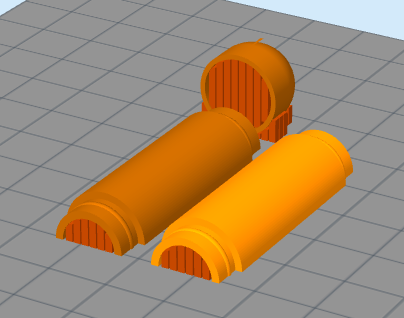
\includegraphics[width=0.6\linewidth]{figures/3d-model}
  \caption{Casing model}
  \label{fig:3d-model}
\end{figure}

\begin{figure}[h]
  \centering
    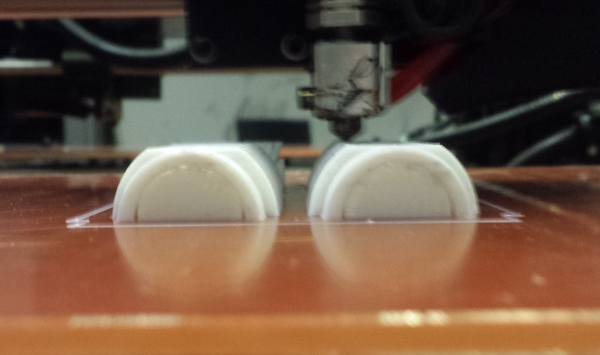
\includegraphics[width=0.6\linewidth]{figures/3d-print}
  \caption{3D printing the casing}
  \label{fig:3d-print}
\end{figure}

\section{Position Reconstruction}
To digitize writing with IMU data, position reconstruction is developed using various methods of post-processing. The reconstruction and plotting code is written in Python with NumPy and MatPlotLib libraries. The code is provided in the appendix.

\subsection{IMU Sensor Data}
	The Bosch IMU provides accelerometer, gyroscope, and magnetometer data. The on-chip Sensortec sensor fusion subtracts the gravity vector to provide linear acceleration. It also uses proprietary algorithms to fuse all nine degrees of freedom for more reliable data. The sensor fusion with the gyroscope and the magnetometer provide absolute orientation to North as well as gyroscope stability. From this, we are able to use the Euler angles in position reconstruction. Yaw (rotation about the z-axis) and pitch (rotation about the y-axis) have ranges of 360 degrees, whereas roll (rotation about the x-axis) has a range of 180 degrees.

\subsection{Filtering and Thresholding}
  Once the LightBlue Bean has transmitted the IMU data, we must filter it because the on-chip sensor fusion is not accurate enough for position reconstruction. First, we noted that the IMU calibration was not always perfect. Fig. 8a shows the raw data obtained from the IMU on a trial run when it is stationary. As seen by the green line in the plot, the data drifts and gets periodically recalibrated around once every 10 seconds. To solve this issue, we implemented a high pass filter by subtracting the reading from some mean value computed through a low-pass infinite impulse response (IIR) filter with a very low cutoff frequency. The high-pass filter eliminates this offset as seen in Fig. 8b.
\par Next, we implemented an IIR low pass filter, which significantly reduces the noise as shown in Fig. 8c.
  Lastly, we implemented acceleration thresholding: if the measured acceleration is under a certain threshold, we assume it is due to noise and ignore it. Unfortunately, this thresholding makes it difficult to recognize slow movement. Therefore, we require the user to write with fast movements. The effects are seen in Fig. 8d.
\begin{figure}[h]
  \centering
    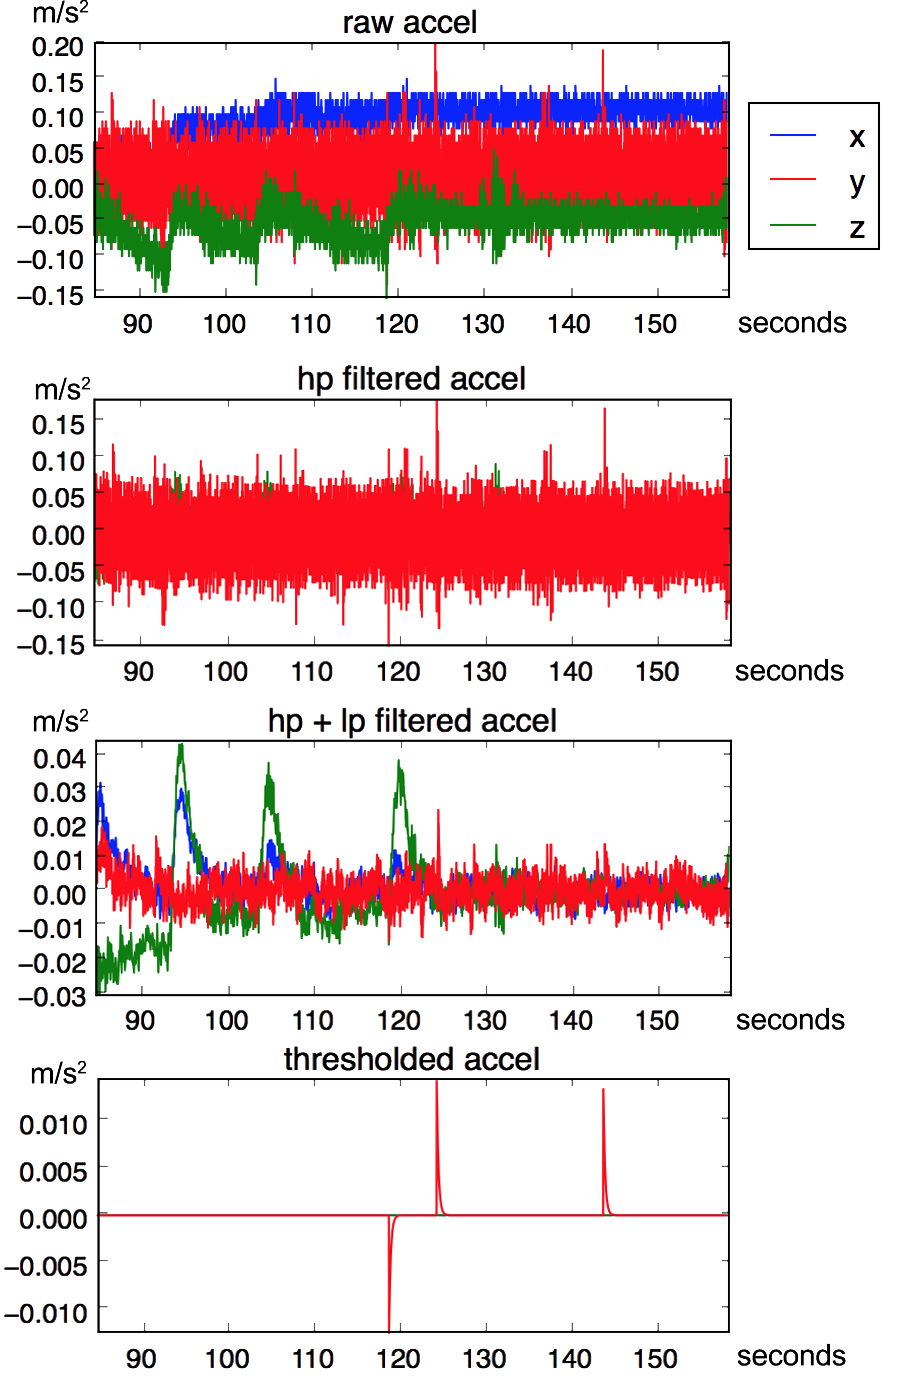
\includegraphics[width=0.9\linewidth]{figures/filtering}
  \caption{(a) Raw data from IMU; (b) Processed with high pass filter; (c) Processed with low pass filter; (d) Thresholded}
  \label{fig:filtering}
\end{figure}

\subsection{Transformation to Fixed Reference Frame}
  Since the acceleration data is provided in the IMU reference frame, we need to perform a change of basis to real world coordinates. The first position recorded is chosen to be the new fixed frame of reference. To perform this basis transformation, we used the Directional Cosine Matrix from \cite{PB}. $Q_G$ is the coordinate system from the fixed reference frame while $Q_P$ is the coordinate system from the IMU reference frame.

\begin{figure}[h]
  \centering
    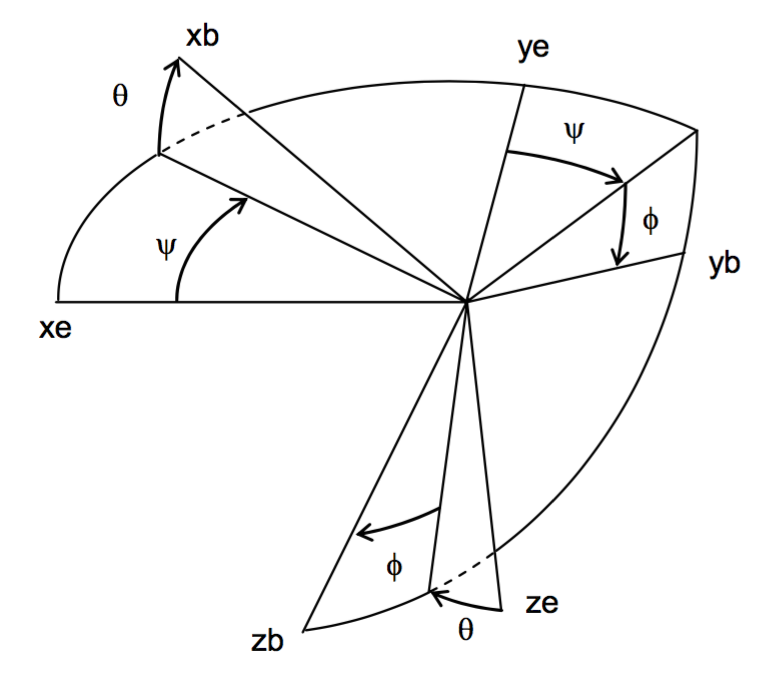
\includegraphics[width=\linewidth]{figures/dcm}
  \caption{Angles corresponding to the DCM [Premerlani and Bizard]}
  \label{fig:vel-adjust}
\end{figure}

\subsection{Velocity Adjustment}
	We discovered that we needed to adjust velocity. When acceleration is near zero for some period of time, it is highly likely that the marker is stationary. The IMU data is imperfect. This causes the velocity to be nonzero as shown in Fig. 10a, which shows velocity reconstruction for a step in the y-axis direction.
\par To counter this issue, we assumed that if absolute acceleration is within some small bound for a set time, the velocity should be zero. Then we shift the velocity towards zero by comparing its current value to its value the first and last time the acceleration left the acceleration bounds near zero. Assuming $i$ is the index when the acceleration leaves the bounds and $j$ is the index when the acceleration enters the bounds, the velocity warping formula we used is shown below:
$$v_{\text{adjusted}}[n] = v_{\text{unadjusted}}[n] - \left(\frac{n-i}{j-i}\right)^2 v_{\text{unadjusted}}[j]$$
This algorithm is executed on the three axes of movements independent of each other. The resulting velocity is shown in Fig. 10b.

\begin{figure}[h]
  \centering
    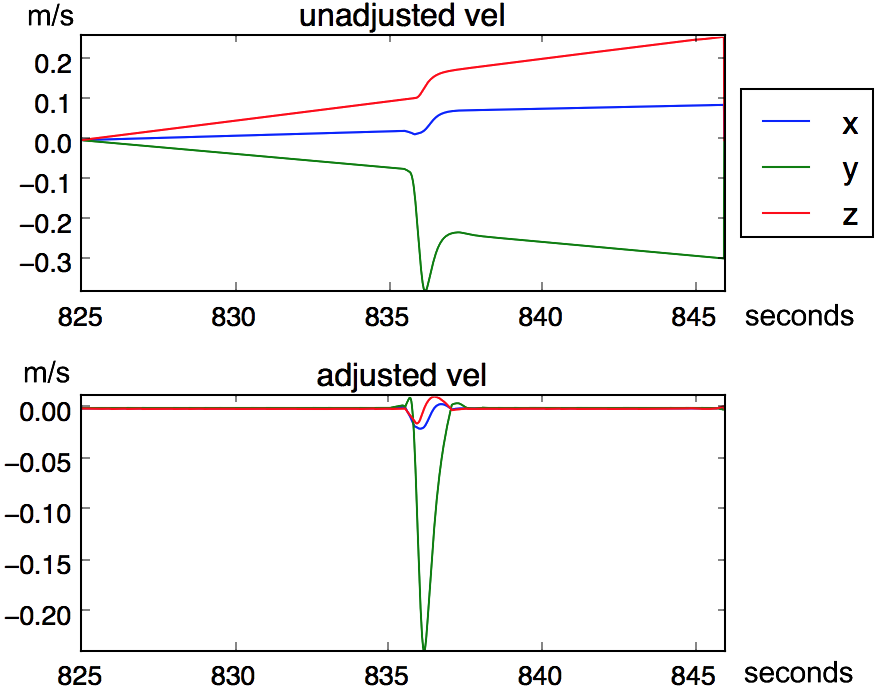
\includegraphics[width=0.9\linewidth]{figures/vel-adjust}
  \caption{(a) Velocity integrated from acceleration data; (b) After velocity adjustment}
  \label{fig:vel-adjust}
\end{figure}

\subsection{Tip Position Reconstruction}
Because the IMU was mounted on the end cap of the casing, we used the Euler angles and the marker length to compute the position of the tip. The yaw reading from the IMU did not matter because we draw on a 2D-plane and the marker is assumed to be along the z-axis of the IMU. We calculated that, if the reconstructed position of the IMU is $(x,y)$, the tip position is $(x-sin(pitch), y-sin(roll))$.

\subsection{Plotting}
  The position is plotted after reconstruction. We perform the post-processing every 20 data points to reduce latency since NumPy uses vector computations. If the force sensor is turned off during one of the last 20 data points, the plot is updated to include the last stroke. Although we reconstruct position for all transmitted data, we only plot when the force sensor is pressed. We also clear the position plot if button is pressed. 

\section{Quantitative Analysis and Scheduling}
Scheduling was another challenge we encountered. The Bean provides the Arduino serial library through a virtual serial port, but it has a very limited data rate. The worst case execution time (WCET) for each block of the most naive version of the Arduino code is shown in the Control Flow Graph (CFG) in Fig. 11. Through this quantitative analysis, we discovered that sending data over Serial.println() was infeasible since it converts numbers into numerical characters, and each order of magnitude takes a whole byte of character space. The timing was inferred by setting a digital output pin high before and low after a block of code. We used an oscilloscope to measure the time the digital output pin is high. This assumes that the time to write to the pins is negligible.
\begin{figure}[h]
  \centering
    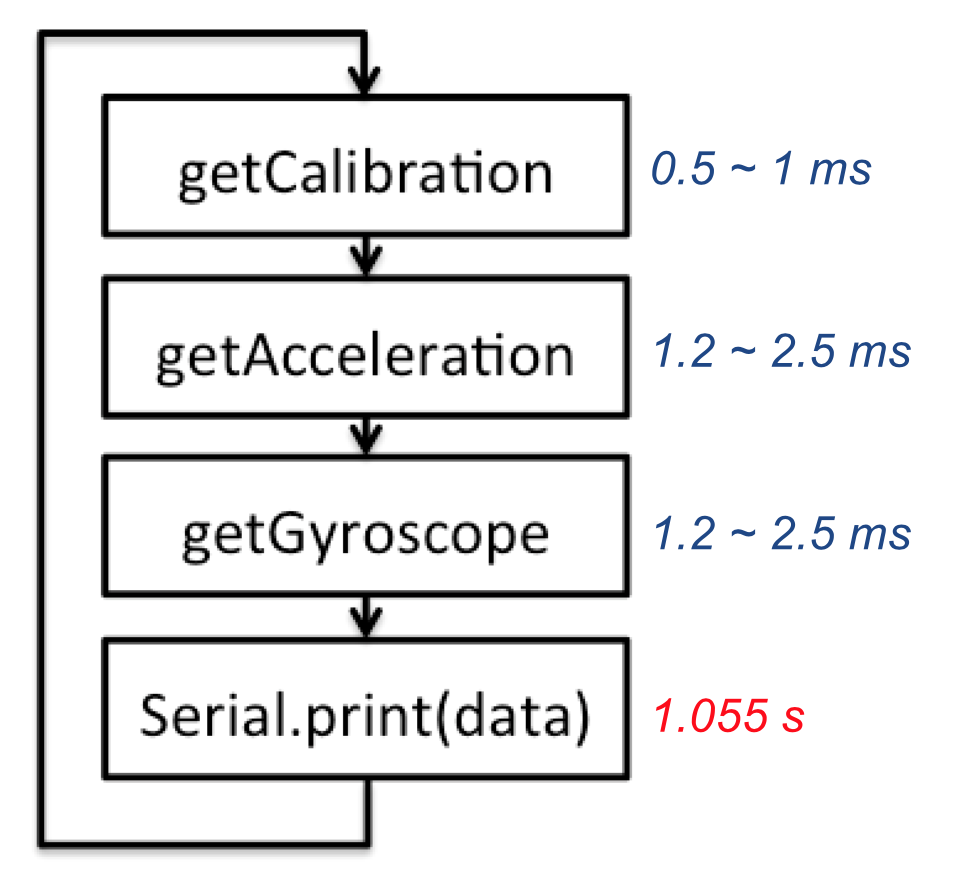
\includegraphics[width=0.6\linewidth]{figures/cfg1}
  \caption{CFG1: Naive implementation of microcontroller code with Serial.println()}
  \label{fig:cfg1}
\end{figure}

\par To make scheduling feasible, we switched from using Serial.println() to Serial.write() for sending bytes instead of characters. We discovered that the serial communication is implemented by sending 64 bytes of data in each message payload, so we send five 12 byte custom data packets per message. Once the IMU is calibrated, we send data packets with a set valid bit and assume the IMU will stay calibrated. Until then, only calibration data is sent to the PC. As shown in Fig. 12, this takes about 24 ms for each payload; however, every sixth packet is dropped since from a scheduling point of view one in every six tasks of getting the data and setting the buffer is infeasible due to the Serial.write() call. The function call cannot be preempted with reasonable effort, but this is an acceptable issue because the sampling rate is fast enough for our purposes. While waiting for enough data to send, the current data is pushed into a buffer which acts like a FIFO that triggers when capacity is reached and sends the data.
\begin{figure}[h]
  \centering
    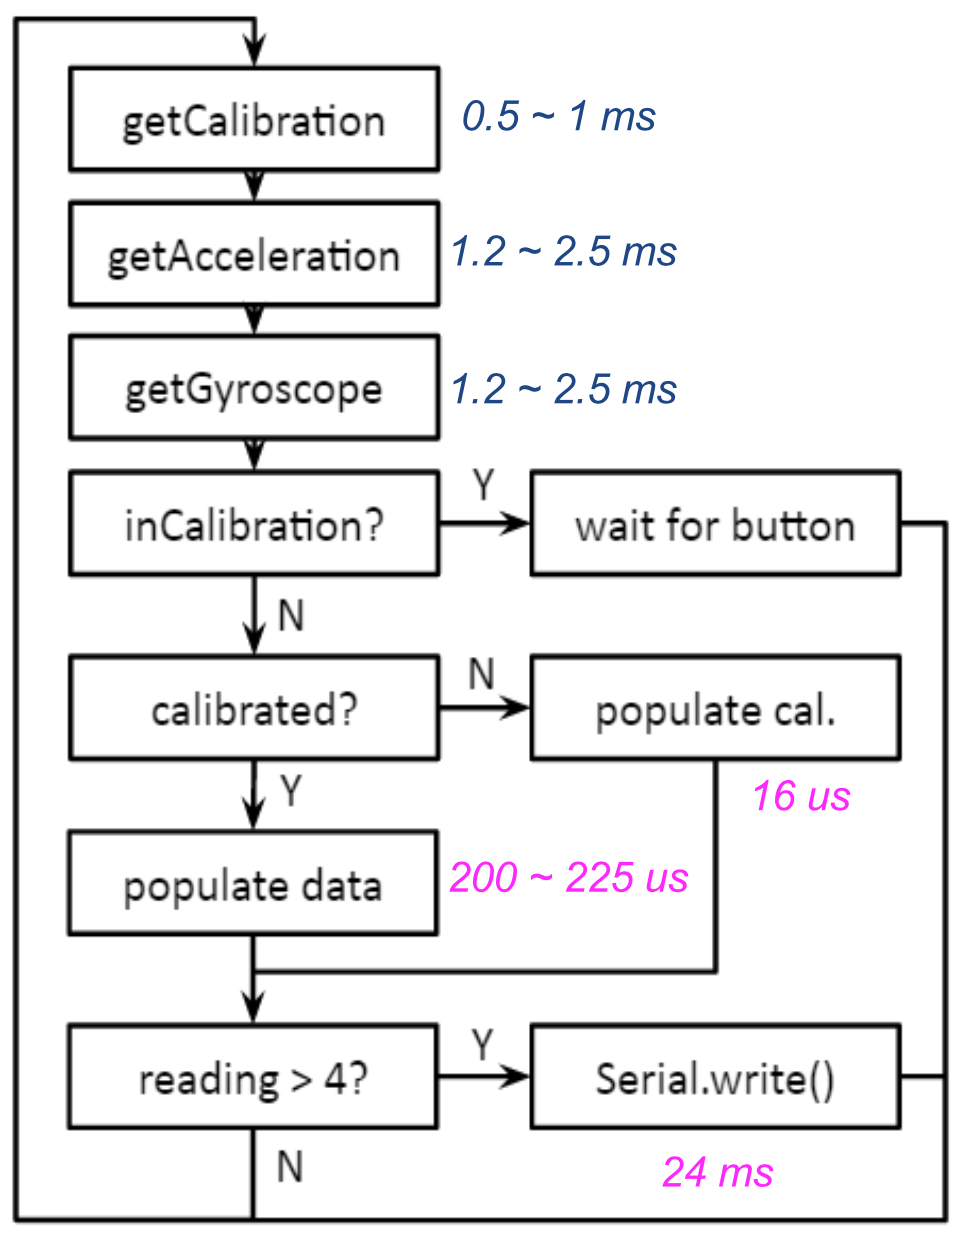
\includegraphics[width=0.8\linewidth]{figures/cfg2}
  \caption{CFG2: Optimized implementation of microcontroller code with Serial.write() and custom data packets}
  \label{fig:cfg2}
\end{figure}

\par Additionally, the Bean's RGB LED is controlled by the BLE module in the Bean instead of the microcontroller, so it takes about 30 ms to set the LED color which is equivalent to two dropped readings per LED setting. To solve this issue, we switched to the LED sequin, which only uses a digitalWrite() function call since it is a digital output pin controlled by the microcontroller. 
  

\subsection{Custom Data Packets}
Each of our custom data packets contains 5 readings of 12 bytes. The purpose of each bit can be seen in Fig. 13. The valid bit is used to signify that the IMU is fully calibrated. Three bits are assigned to buttons and the force sensor depending on their on or off status (one of these is unused in the current prototype). Each axis of acceleration has 12 bits encoded which allows for an acceleration range of -20.48 to 20.47 $m/s^2$ with 2 decimal places in each axis. Sixteen bits are assigned to each axis of the Gyroscope to allow for a range of -180.00 to 180.00 degrees with 2 decimal places. The last eight bits contain a counter to help with detecting packet loss during the reconstruction.

\begin{figure}[h]
  \centering
    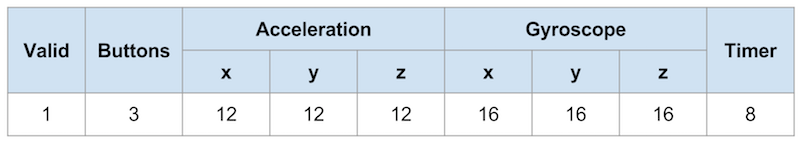
\includegraphics[width=\linewidth]{figures/packet}
  		\caption{Custom Data Packet}
  	\label{fig:packet}
\end{figure}

\section{Mode of Operation}
reWRITE can be modeled by the hierarchical state machine in Fig. 14. When reWRITE is turned on, it enters the ‘Calibration' state. In this state, the IMU calibrates the accelerometer, gyroscope, and magnetometer, and prints each level of calibration. When all three sensors are calibrated, reWRITE preemptively transitions and enters the ‘Button' state. Here, it waits for the user to press the button before starting position reconstruction. Once the button is pressed, reWRITE enters the ‘Data' state. The nested state machine in ‘Data' is also a hierarchical state machine. In ‘Data', the system constantly receives new data and plots the reconstructed position. It performs calculations and plots by utilizing synchronous composition of state machines in the ‘Active' state. One of the synchronous state machines executes the velocity calibration when the guard evaluates to true. Simultaneously, the other state machine plots the position when the marker presses the force sensor.

\begin{figure}[h]
  \centering
    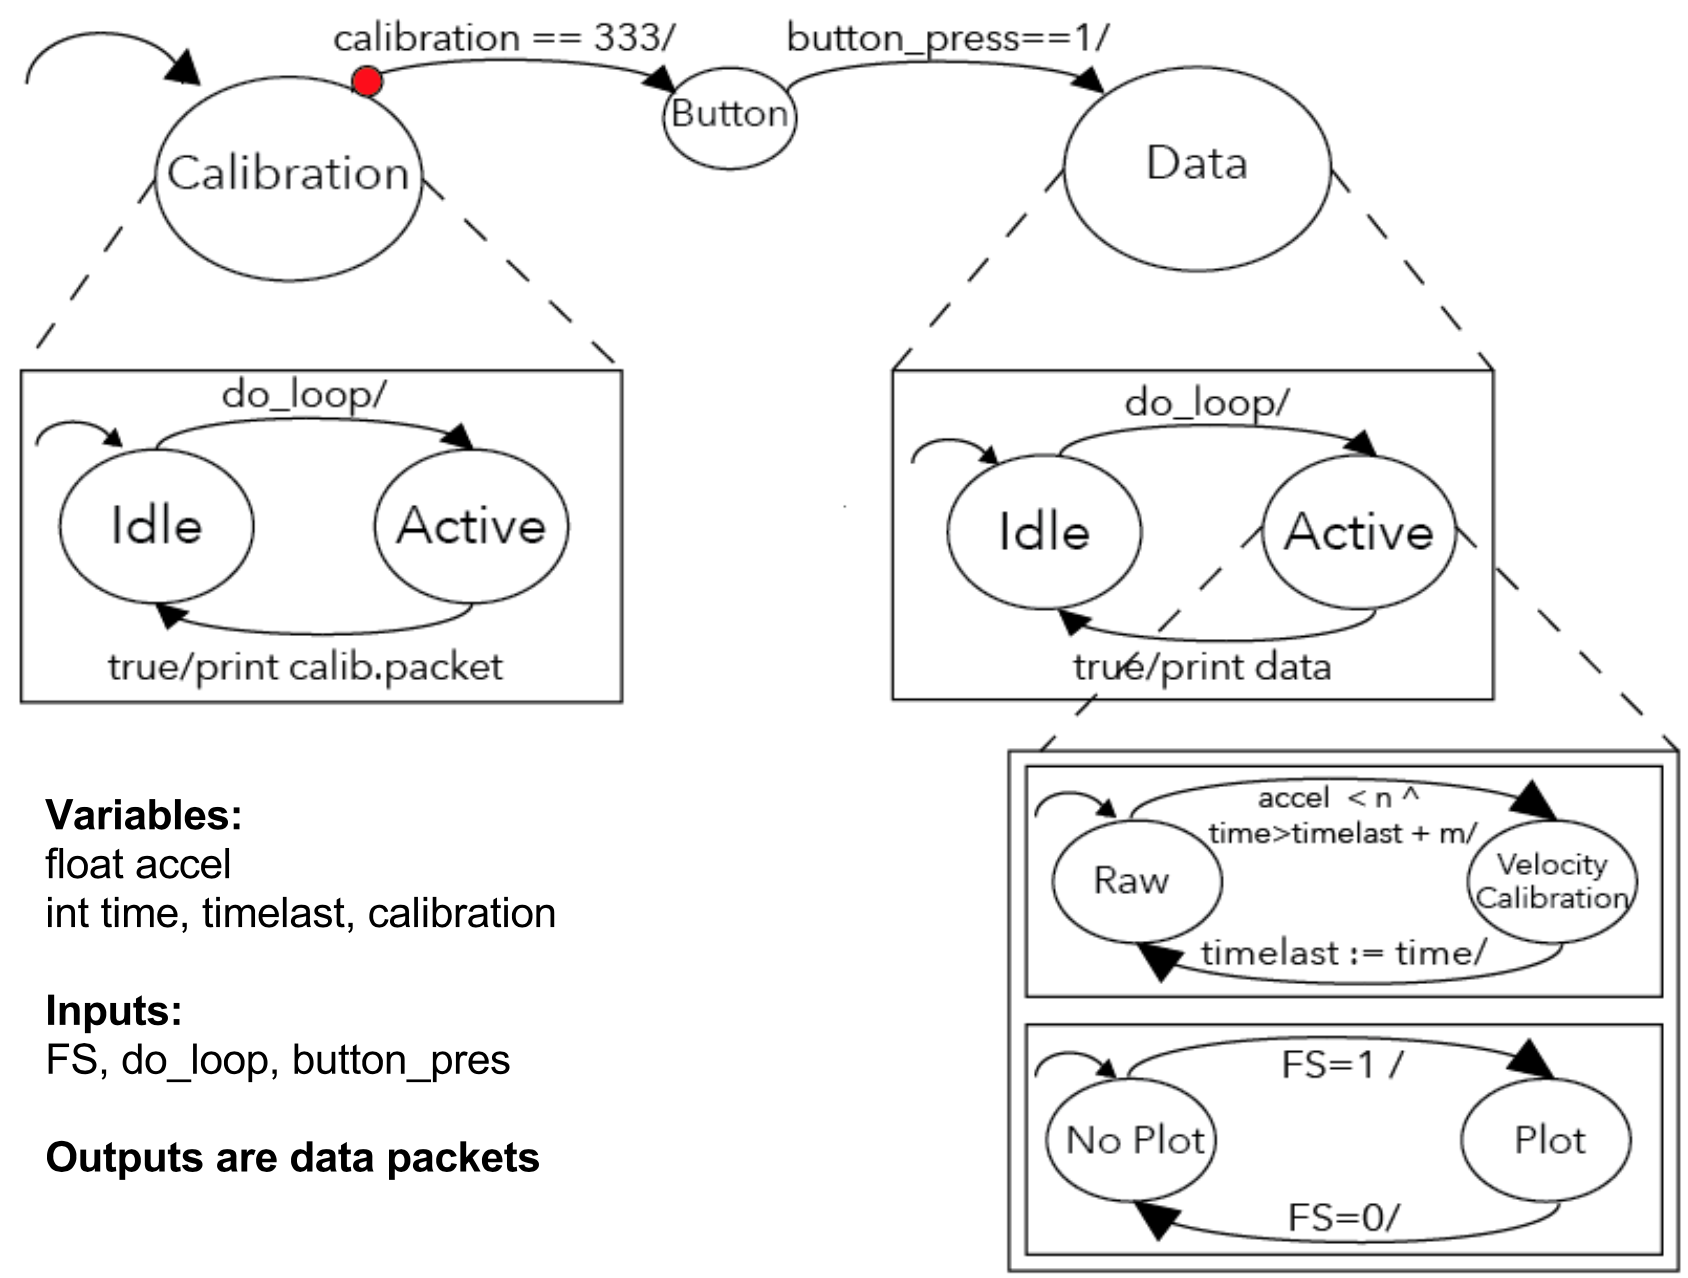
\includegraphics[width=\linewidth]{figures/fsm}
  \caption{Finite State Machine}
  \label{fig:fsm}
\end{figure}

\section{Bill of Materials}
%\centering
\begin{tabular}{r|l}
Component & Price \\
\hline
LightBlue Bean & \$30 \\
BNO055 Absolute Orientation Sensor & \$35 \\
Li-Ion 3.7V 150mAh Battery and Charger & \$13 \\
Force Sensor & \$7 \\
Button and LED & \$2 \\
3D Printing & \$2 \\
\hline
Total & \$89 \\
\end{tabular}

\section{Acknowledgements}
We would like to acknowledge the following individuals for their support and contribution in this project.
\begin{itemize}
\item Trung Tran, \textit{National Instruments}
\item Prof. Sanjit Seshia, \textit{UC Berkeley}
\item Matthew Weber, \textit{UC Berkeley}
\item Eric Kim, \textit{UC Berkeley}
\item Casey Rogers, \textit{UC Berkeley 3D Modeling Club}
\end{itemize}

\begin{thebibliography}{1}
\bibitem{PB} Premerlani, W., Bizard, P.: Direction cosine matrix	IMU: theory. http://gentlenav.googlecode.com/files/DCMDraft2.pdf
\end{thebibliography}

\newpage
\onecolumn

\section{Appendix 1: LightBlue Bean code}
\small{
\lstinputlisting[language=C,frame=single,breaklines=true]{stream_data.ino}
}

\section{Appendix 2: Python code}
\small{
\lstinputlisting[language=Python,frame=single,breaklines=true]{draw.py}
}

\end{document}



